\chapter{Methode}
\section{Experiment en instrumentatie}
Voor het valideren van het voorgestelde model wordt gebruik gemaakt van een opstelling waarbij twee magneten boven elkaar hangen zie Figuur \ref{fig:IE1:opstelling}. Daarbij wordt de onderlinge kracht tussen de magneten op verschillende hart-tot-hart afstanden bepaald.

\begin{figure}[H]
    \centering
    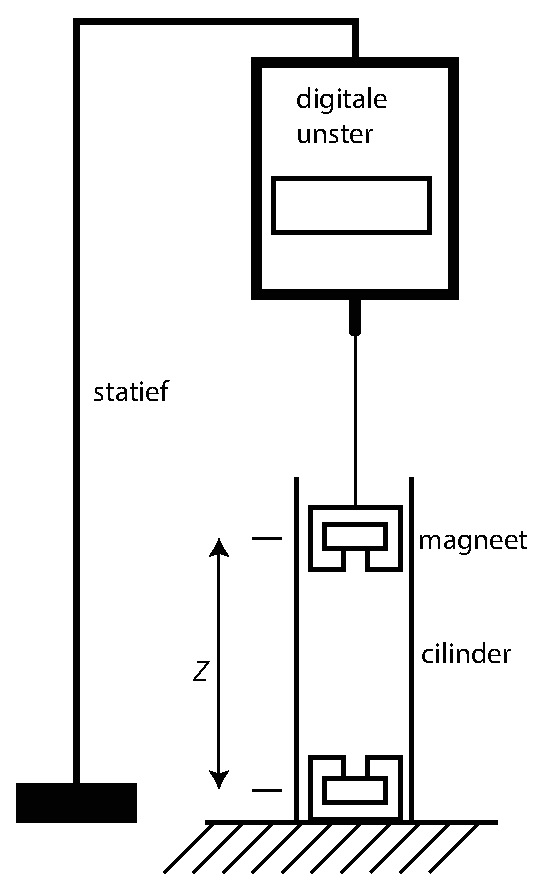
\includegraphics[width=0.4\textwidth]{Figures/IE1_opstelling.eps}
    \caption{In de opstelling voor de bepaling van de kracht tussen twee magneten wordt de onderlinge kracht bepaald m.b.v. een digitale unster.}
    \label{fig:IE1:opstelling}
\end{figure}
De hart-tot-hart afstand (Figuur \ref{fig:IE1:opstellingr}) tussen de twee magneten wordt gegeven door:
\begin{equation}
    z = \frac{1}{2}d_m+h_1+h_{1,2}+h_2+\frac{1}{2} d_m
\end{equation}
\begin{figure}
    \centering
    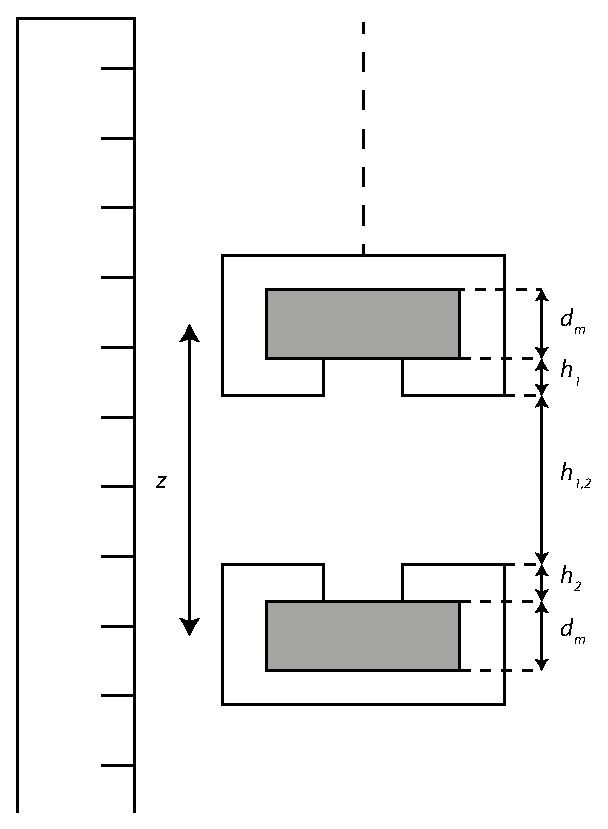
\includegraphics[width=0.5\textwidth]{Figures/ie1_opst_onz.eps}
    \caption{De opstelling bestaat uit twee magneten met een hart-tot-hart afstand $z$.}
    \label{fig:IE1:opstellingr}
\end{figure}

Voor bepaling van $h_1$ en $h_2$ wordt een schuifmaat gebruikt met een meetonzekerheid van 0.5 mm, $h_{1,2}$ wordt bepaald m.b.v. een liniaal met een meetonzekerheid van 5 mm. Volgens de specificatie van de magneet is de meetonzekerheid in de diameter van de magneet X mm (GmbH, 2011). Dit levert een totaal meetonzekerheid van $\mu_z$= X mm. Zie de Appendix voor de bijbehorende afleiding.\\
Met behulp van een digitale unster (Christen Orange OR-42) met een aflees-nauwkeurigheid van 1 g wordt de onderlinge uitgeoefende kracht bepaald:
\begin{equation}
    F_{1,2}=\Delta m \cdot g
\end{equation}
hierin is $g$ de zwaartekrachtsversnelling in Nederland met een waarde van 9,812 $\pm$ 0,001 m/s$^{2}$ en $\Delta m$ het verschil in massa in kg gegeven door:
\begin{equation}
    \Delta m=m_\infty-m_z			
\end{equation}
Aangezien de meetonzekerheid in $g$ velen malen kleiner is dan de meetonzekerheid in $m$, geldt $\mu_F$ = 1·10$^{-2}$ N, zie de appendix voor de afleiding.

\section{Procedure}